\lecture{26}{2025-05-21}{almost the end}{}
\begin{parag}{How to decode}
    Hence the coseet decoder can be implemented as follows:
    \begin{enumerate}
        \item We precompute and store the coset leaders and the corresponding syndrome
        \item To decode $y$, we compute its syndrom $s = yH^T$
        \item $s$ encodes the row of $y$
        \item We use the lookup table to determine the corresponding coset leader, say, $t_i$
        \item $t_i$ and $y$ uniquely determine the column of $y$ namely $y =  t_i + c_j$
           \item hence $c_j =  y - t_i$
           \item the decoder  declares
    \end{enumerate}
    
\end{parag}


\begin{parag}{Choosing coset leaders}
   \begin{subparag}{Rule ``MD''}
       In every coset, the leader is the minimum weight sequence.
   \end{subparag}
   \begin{theoreme}
   The coset decoder is a minimum distance decoder
   \end{theoreme}
   \begin{subparag}{Proof}
       Suppose $\vec{y}$ is in row $i$ , column $j$ of the standard array. We know then $\vec{y} =  \vec{c}_j + \vec{t}_i$.\\
       Then we know that the coset decoder will:
       \begin{itemize}
           \item decode: $\vec{y} \to \vec{c}_j$
           \item Hence $d\left(\vec{y}, \vec{c}_j\right) =  w\left(\vec{t}_i\right)$
       \end{itemize}
       Now consider any $\vec{c}_k$:
       \begin{align*} 
           d\left(\vec{y}, \vec{c}_k\right) &= w\left(\vec{y} - \vec{c}_k\right)\\
                                     &= w\left(\vec{c}_j + \vec{t}_i - \vec{c}_k\right)\\
                                     &= w\left(\left(\vec{c}_k - \vec{c}_k\right) + \vec{t}_i\right)
       \end{align*}
       Now the question is: who is the leader of this?\\
       We know because of $\vec{t}_i$ we know that we are in the row $i$.\\
       Then we want to show that $d\left(\vec{y}, \vec{c}_k\right) \geq w\left(\vec{t}_i\right)$.\\
       By construction, we choose the coset leader by the one who is the lowest weight. Then as we said before we know that $d\left(\vec{y}, \vec{c}_k\right) = w\left(\vec{c}_j - \vec{c}_k +\vec{t}_i\right)$ which is also in row $i$. And because $\vec{t}_i$ is the lowest weight then it has to be lower than $d\left(\vec{y}, \vec{c}_k\right)$.
   \end{subparag}
\end{parag}


\begin{parag}{Example ($\left(6, 3\right)$ binary linear block code) }

    The code is defined by the following parity check matrix:
    \begin{align*} 
        H =  \begin{pmatrix} 0&1  & 1 & 1 & 0 & 0 \\ 1 & 0 & 1 & 0 & 1 & 0 \\ 1 & 1 & 0 & 0 & 0 &  \end{pmatrix} 
    \end{align*}
    We can see here that    two columns are linearly dependent. The first three columns are linearly dependent. Hence $d_{min} =  3$.\\
    $H$ hat the form $\left(P, I\right)$, The generator matrix $G$ has the form $\left(I,-P^T\right)$
    \begin{align*} 
        G = \begin{pmatrix} 1 & 0 & 0 & 0 & 1 & 1 \\ 0 & 1 & 0 & 1 & 0 & 1 \\ 0 & 0 & 1 & 1 & 1 & 0  \end{pmatrix} 
    \end{align*}

\end{parag}



\begin{parag}{Error probability}
    There are many ways to choose $\mathcal{D}_0$.  In fact every element of every row of the standard array can be chosen as the coset leader. Next, we learn how to choose the coser leaders so as to minimize the decoding error-probability.\\
    Suppose that the channel is the following binary symmetric channel with input alphabet $\mathcal{X} = \left\{0, 1\right\}$ and output alphabet $\mathcal{Y} = \left\{0, 1\right\}$. (Binary symmetric channel)
    \begin{center}
        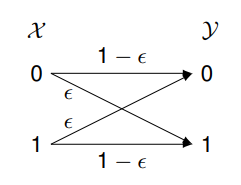
\includegraphics[scale=0.8]{12025-05-21.png}
    \end{center}
    We tale $\vec{e}$ a string of \important{independent} binaries with $P\left(e_i =  1\right) =  \epsilon$, hence what is:
    \begin{align*} 
        P\left(\vec{e} &=  \left(0, 1, 0, 0, 1, 0, 1\right)\right) = p\left(e_i= 0\right)p\left(e_2= 1\right)\ldots\\
                        &= \left(1-\epsilon\right)\epsilon\left(1-\epsilon\right)\ldots\\
                        &= \left(1-\epsilon\right)^{\text{nbr of zeroes}}\cdot \epsilon^{\text{nbr of ones}}\\
                        &= \left(1-\epsilon\right)^4\epsilon^3 
    \end{align*}
    We know that in a sequence $\vec{e}$ the number of one:
\begin{align*} nbr_1 =  w\left(\vec{e}\right) \end{align*}
And for the number of zeroes:
\begin{align*} 
    nbr_0 =  n - w\left(\vec{e}\right)
\end{align*}
Then we can see that:
\begin{formule}
\begin{align*} 
    P\left(\vec{e}\right) &=  \left(1-\epsilon\right)^{n-w\left(\vec{e}\right)}\epsilon^{w\left(\vec{e}\right)}\\
    &= \left(1-\epsilon\right)^n\left(\frac{\epsilon}{1-\epsilon}\right)^{w\left(\vec{e}\right)}
\end{align*}
\end{formule}
    
In a lot of exercise and exam question, it is easier to use the probability the we decode \important{correctly} the given code.\\
We start by taking $\vec{c}_0 = \vec{0}$, we then look for $P_c\left(0\right) =  P\left(\text{error pattern was ``good''}\right)$
Then:
\begin{align*} 
    =p\left(\text{ error pattern is one from the column below} \vec{c}_0\right)\\
    = p\left(\vec{e} \in \mathcal{D}_0\right)\\
    = \sum_{e \in \mathcal{D}_0} p\left(\vec{e}\right)\\
    = \sum_{\vec{e}\in \mathcal{D}_0}\left(1-\epsilon\right)^{n-w\left(e\right)}\epsilon^{w\left(e\right)}
\end{align*}
In other words, when $c_0 \in \mathcal{C}$ is transmitted, the decoder makes the correct decision whenever $y \in \mathcal{D}_0$. But when $c_0$ is transmitted, the event $y \in \mathcal{D}_0$ is the same as the event $e \in \mathcal{D}_0$. 
\begin{framedremark}
What we do to comput the probability we do the sum over all elements of the column with the exact weight... This  can be said like this:
\begin{align*} P_C\left(0\right) =  \sum_{j= 0}^{L-1} \epsilon^{w\left(t_j\right)}\left(1-\epsilon\right)^{n-w\left(t_j\right)} \end{align*}
\end{framedremark}
\end{parag}


\begin{parag}{Next}
    Now, what if $\vec{c}_i$ is the transmitted codeword?
    \begin{align*} 
        P_c\left(i\right) &= P\left(\vec{y} \in \mathcal{D}_i\right)\\
                          &= P\left(\vec{c}_i + \vec{e} \in \mathcal{D}_i\right)
                          &= P\left(\vec{c}_i + \vec{e} \in \vec{c}_i + \mathcal{D}_0\right)\\
                          &= P\left(\vec{e} \in \mathcal{D}_0\right)
    \end{align*}
    What is the probability to make an error if it is $111000$\\
    We have assumed for simplicity a binary symmetric channel, but the same idea applies to nonbinary channel (with input and output alphabet $\mathbb{F}$) for which the probability of an error pattern $e \in \mathbb{F}^n$ is decreasing with $w\left(e\right)$\\
    $P_C\left(c_i\right)$ is the probability that $y \in \mathcal{D}_i$ when $c_i$ is transmitted\\
    This is the probability that $\underbrace{c_i + e}_{y} \in \underbrace{c_i + \mathcal{D}_0}_{\mathcal{D}_i}$.\\
    Hence, for all $i, P_C\left(c_i\right) =  P_C\left(0\right)$\\
    Hence, the unconditional probability of correct decoding is $P_C = P_C\left(0\right)$
\end{parag}


\section{Reed Solomon Codes}



\begin{parag}{Polynomials over finite fields}
    Not surprisingly, the notion of polynomial extends to finite fields.
    \begin{itemize}
        \item let $\vec{u} =  \left(u_1, \ldots, u_k\right)$ for some finite field $F$
        \item We associate to $\vec{u}$ the polynomial:
           \begin{align*} P_{\vec{u}}\left(x\right) =  u_1 + u_2x + \cdots + u_kx^{k-1}  \end{align*}
       \item $P_{\vec{u}}\left(x\right)$ can be evaluated at any $x \in \mathbb{F}$
       \item The degree of a polynomial is the highest exponent $i$ for which $x^i$ has a non-zero coefficient.
       \item By convention, the zero polynomial has degree $-\infty$.
    \end{itemize}
   \begin{subparag}{Example}
       \begin{itemize}
           \item $\mathbb{F} =  \mathbb{F}_5$ 
           \item $P\left(x\right) =  2 + 4x + 3x^2$ is a polynomial of degree 2 over $\mathbb{F}$
           \item $P\left(x\right) =  P_{\vec{u}}\left(x\right)$ for $\vec{u} = \left(2, 4, 3\right) \in \mathbb{F}_5^3$
           \item A polynomial $P\left(x\right)$ over a field $\mathbb{F}$ can be evaluated at any $x \in \mathbb{F}$:
               \begin{align*} P_{\vec{u}}\left(2\right) = 2 + 4\cdot 2 + 3 \cdot 2^2 = 2 + 3 +  2 = 2\end{align*}
       \end{itemize}  
       
   \end{subparag} 
\end{parag}


\begin{parag}{Interpolation via polynomials}
    Problem: given a field $\mathbb{F}$ and $k$ pairs $\left(a_i, y_i\right) \in \mathbb{F}^2$, where the $a_i$ are all distinct is there a polynomial $P\left(X\right)$ over $\mathbb{F}$ of degree at most $k-1$ (hence described by at most $k$ coefficients) such that:
    \begin{align*} 
        P\left(a_i\right) =  y_i, \;\; i =  1, \ldots, k
    \end{align*}
    \begin{center}
        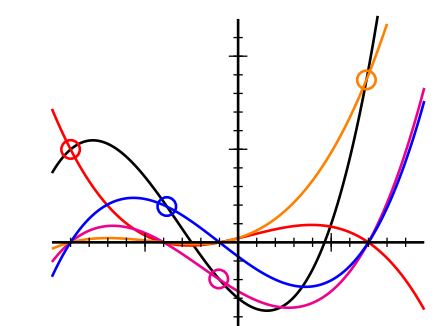
\includegraphics[scale=0.8]{32025-05-21.png}
    \end{center}
    
\end{parag}
\begin{parag}{Lagrange's interpolation polynomials}
   To simplify notation, we demonstrate how it works by means of examples:
   \begin{subparag}{Example}
       \begin{itemize}
           \item Fix a field $\mathbb{F}$ and distinct field elements $a_1, a_2, a_3$ as well as $y_1, y_2, y_3$ (not necessarily distinct)
           \item We seek polynomial $P\left(x\right)$ of degree at most $2$ and coefficient in $\mathbb{F}$ such that $P\left(a_i\right) =  y_i$
           \item Suppose we can find a polynomial $Q_1\left(x\right)$ of degree at most 2 such that:
       \end{itemize}
       
   \end{subparag}
\end{parag}

